% =====================================================================
% Plantilla de respuestas · Tarea Computacional · IMT2220 (2026-2)
% =====================================================================
% Cómo usarla:
%   1. Completen el número de grupo y los integrantes (más abajo).
%   2. Reemplacen cada \pendiente por su desarrollo y su respuesta.
%   3. Las figuras que guarden desde sus notebooks van en la carpeta figuras/.
%   4. Compilen con pdfLaTeX (en Overleaf es el compilador por defecto) o con LuaLaTeX.
%
% En Overleaf: New Project > Upload Project y suban el .zip con esta carpeta.
% Pueden borrar estos comentarios y las cajas de "Indicaciones" cuando terminen.
\documentclass{article}
\usepackage{plantilla}
\graphicspath{{figuras/}}
\settitulo{Tarea Computacional}

% ---------------------------------------------------------------------
% Datos del grupo
% ---------------------------------------------------------------------
\newcommand\grupo{2}   % <-- número del grupo
\integrantes{%
  Alondra Estay \\
  Gaspar Galaz \\
  José Mora \\
  Renato Reyes}

% Marca para lo que falta por completar (búsquenla con Ctrl+F antes de entregar)
\newcommand\pendiente{{\color{gris90}\itshape [Escriban aquí su desarrollo y su respuesta.]}}

\begin{document}

\portada[Grupo \grupo]

% =====================================================================
\seccionsinnumero{Indicaciones para usar esta plantilla}
% =====================================================================

\begin{nota}[Indicaciones]
  Esta plantilla es recomendada para resolver la tarea (aunque pueden utilizar cualquier otro formato mientras cumplan con lo solicitado).
  Pueden reemplazar cada \pendiente{} por su desarrollo.
  Al final de este archivo hay ejemplos de cómo escribir ecuaciones, incluir figuras y tablas. Borren esa página antes de entregar.
\end{nota}

Algunas recomendaciones
\begin{itemize}
  \item \textbf{Desarrollo.} Justifiquen cada paso: no basta con el resultado. Cuando usen un resultado de clases, menciónenlo.
  \item \textbf{Resultados numéricos.} Reporten los valores que se piden (normas, residuos, $J(\theta)$, etc.) con 3 o 4 cifras significativas e indiquen de qué celda del notebook salen. (Esto no es estrictamente necesario, pero sí recomendado.)
  \item \textbf{Figuras.} Guárdenlas desde el notebook con \code{plt.savefig("figuras/nombre.png", dpi=200, bbox\_inches="tight")}, súbanlas a la carpeta \code{figuras/} (para que puedan añadirlas aquí) y comenten lo que se ve en ellas.
\end{itemize}
\despueslista

% =====================================================================
\problema{Reconstrucción de una imagen}
% =====================================================================

\seccion{(a) Mínimos cuadrados}

\begin{enumerate}[label=\roman*., widest=iii]
  \item \textbf{Gradiente y matriz Hessiana de $J_0$.}

  Consideraremos la función:
  \[
  J_0(x)=\|Ax-b\|_2^2
  \]

  \subsubsection*{• Cálculo del gradiente}

  Para calcular el gradiente, primero expandiremos la función utilizando la propiedad de la norma euclidiana al cuadrado, \(\|x\|_2^2=x^Tx\):

  \[
  \begin{aligned}
  J_0(x) &= (Ax-b)^T(Ax-b)\\
  &=x^TA^TAx-x^TA^Tb-b^TAx+b^Tb
  \end{aligned}
  \]

  Como \(x^TA^Tb\) es un escalar, es igual a su transpuesta, es decir, \(x^TA^Tb=(x^TA^Tb)^T=b^TAx\).

  Al tener esto en consideración, podemos agrupar los términos del medio y obtener:

  \[
  J_0(x)=x^TA^TAx-2x^TA^Tb+b^Tb
  \]

  Con la función expresada de esta forma, podemos calcular su gradiente derivando cada término respecto del vector \(x\). Realizando la derivación, obtenemos que el gradiente de \(J_0\) es:

  \[
  \boxed{\nabla J_0(x)=2A^T(Ax-b)}
  \]

  \subsubsection*{• Cálculo de la Matriz Hessiana}

  Para calcular la matriz Hessiana, debemos encontrar las segundas derivadas parciales de una función. En este caso, como \(J_0(x)\) depende del vector \(x\), podemos obtener la Hessiana derivando el gradiente respecto de \(x\), considerando que las matrices \(A\) y \(A^T\) y el vector \(b\) son constantes.

  Por lo tanto, la matriz Hessiana es:

  \[
  \boxed{H_{J_0}=2A^TA}
  \]

  \bigskip
  \bigskip
  \bigskip
  \bigskip

  \subsubsection*{• Deducción de las ecuaciones normales}

  Para demostrar que los puntos críticos de \(J_0(x)\) corresponden a las soluciones de las ecuaciones normales, debemos recordar que un punto crítico de una función es aquel donde su gradiente es igual a cero. Por lo que utilizaremos el gradiente obtenido anteriormente y lo igualaremos a cero:

  \[
  \nabla J_0(x)=2A^T(Ax-b)=0
  \]

  Simplificamos dividiendo por \(2\) y reordenamos los términos:

  \[
  \begin{aligned}
  A^T(Ax-b)&=0\\
  A^TAx-A^Tb&=0\\
  A^TAx&=A^Tb
  \end{aligned}
  \]

  De esta manera, obtenemos la expresión para las ecuaciones normales:

  \[
  \boxed{A^TAx=A^Tb}
  \]

  Por lo tanto, concluimos que si un vector \(x\) es un punto crítico de \(J_0(x)\), entonces necesariamente satisface las ecuaciones normales.

  \bigskip

  \item \textbf{$H_{J_0}$ es semidefinida positiva y todo punto crítico es un mínimo global.}

  \subsubsection*{• Demostración de la Hessiana semidefinida positiva}

  Para demostrar que una matriz \(H\) es semidefinida positiva, se debe cumplir que \(v^THv\geq 0\) para cualquier vector \(v\in\mathbb{R}^n\).

  Del ítem (a).i, obtuvimos que la matriz Hessiana es: \(H_{J_0}=2A^TA\)

  Dado que \(H_{J_0}\) es simétrica, ya que \((2A^TA)^T=2A^TA\), evaluamos la condición anterior tomando un vector cualquiera \(v\in\mathbb{R}^n\) y reemplazamos los valores:

  \[
  \begin{aligned}
  v^TH_{J_0}v
  &=v^T(2A^TA)v\\
  &=2v^TA^TAv\\
  &=2(Av)^T(Av)\\
  &=2\|Av\|_2^2
  \end{aligned}
  \]

  Sabemos que una norma al cuadrado siempre es mayor o igual a cero. Por lo tanto:

  \[
  \boxed{v^TH_{J_0}v=2\|Av\|_2^2\geq 0}
  \]

  Como esta desigualdad se cumple para cualquier vector \(v\), concluimos que la matriz Hessiana \(H_{J_0}\) es semidefinida positiva.

  \vspace{0.5cm} % Espacio en blanco opcional

  \subsubsection*{• Demostración de que todo punto crítico es un mínimo global}

  Para demostrar que cualquier punto crítico de \(J_0(x)\) es un mínimo global, utilizaremos la aproximación de Taylor de segundo orden. Al ser \(J_0(x)\) una función cuadrática, esta aproximación es exacta y podemos expresarla como:

  \[
  J_0(x)=J_0(x_0)+\nabla J_0(x_0)^T(x-x_0)+\frac{1}{2}(x-x_0)^TH_{J_0}(x-x_0)
  \]

  Considerando \(x_0\) un punto crítico, sabemos que su gradiente es igual a cero, es decir, \(\nabla J_0(x_0)=0\). Teniendo esto en cuenta, podemos simplificar la expresión obteniendo:

  \[
  J_0(x)=J_0(x_0)+\frac{1}{2}(x-x_0)^TH_{J_0}(x-x_0)
  \]

  Además, como demostramos anteriormente que la matriz Hessiana es semidefinida positiva, el término cuadrático es siempre mayor o igual a cero:

  \[
  \frac{1}{2}(x-x_0)^TH_{J_0}(x-x_0)\geq 0
  \]

  De esta manera, obtenemos:

  \[
  \boxed{J_0(x)\geq J_0(x_0)}
  \]

  Con esto podemos deducir que el valor de la función en cualquier punto \(x\) es mayor o igual que su valor en el punto crítico \(x_0\). Por lo tanto, concluimos que todo punto crítico de \(J_0(x)\) es un mínimo global de la función.

  \bigskip

  \item \textbf{Unicidad o infinitos minimizadores.}

  \subsubsection*{• Todos los valores propios de \(A^TA\) son positivos}

  Si todos los valores propios de \(A^TA\) son positivos, entonces esta matriz es definida positiva y, por lo tanto, invertible.

  Del ítem (a).i, sabemos que todos los puntos críticos de \(J_0(x)\) satisfacen las ecuaciones normales:

  \[
  A^TAx=A^Tb
  \]

  Como \(A^TA\) es invertible, multiplicamos ambos lados por su inversa para despejar \(x\):

  \[
  \boxed{x=(A^TA)^{-1}A^Tb}
  \]

  Por lo tanto, las ecuaciones normales tienen una única solución, la cual corresponde a un mínimo global de \(J_0(x)\), según lo demostrado en el ítem (a).ii. Con esto podemos concluir que, cuando todos los valores propios de \(A^TA\) son positivos, la función \(J_0(x)\) tiene un único minimizador global.

  \bigskip

  \subsubsection*{• \(A^TA\) tiene al menos un valor propio nulo}

  Si \(A^TA\) tiene un valor propio igual a cero, entonces existe un vector \(v\neq 0\) tal que \(A^TAv=0\).

  Multiplicando por \(v^T\) y utilizando la propiedad de la norma euclidiana, obtenemos:

  \[
  v^TA^TAv=\|Av\|_2^2=0
  \]

  Como una norma solo es cero cuando el vector es nulo, concluimos que \(Av=0\).

  Para demostrar que existen infinitos minimizadores, consideramos un punto crítico \(x_0\) de \(J_0(x)\), que por lo demostrado en el ítem (a).ii también es un mínimo global. A partir de este punto, podemos construir nuevos vectores de la forma \(x_t=x_0+tv\), con \(t\in\mathbb{R}\). Para comprobar si estos también son minimizadores, los reemplazamos en la función:

  \[
  \begin{aligned}
  J_0(x_t)
  &=\|A(x_0+tv)-b\|_2^2\\
  &=\|Ax_0+tAv-b\|_2^2\\
  &=\|Ax_0-b\|_2^2\\
  &=J_0(x_0)
  \end{aligned}
  \]

  Como \(Av=0\), todos los vectores \(x_t\) entregan el mismo valor de la función que \(x_0\), por lo que también son mínimos globales. Además, como \(v\neq 0\) y \(t\) puede tomar infinitos valores, podemos generar infinitos vectores distintos. Por lo tanto, concluimos que, si \(A^TA\) tiene al menos un valor propio nulo, la función \(J_0(x)\) tiene infinitos minimizadores globales.
\end{enumerate}
\despueslista

\seccion{(b) Reconstrucción}

\begin{enumerate}[label=\roman*., widest=ii]
  \item \textbf{Implementación.} Reporten $\norm{x_0}_2$, $\max_i \abs{x_{0,i}}$ y $\norm{Ax_0 - b}_2$, muestren lado a lado $b$ y $x_0$, y respondan las preguntas.

  \begin{figure}[H]
    \centering
    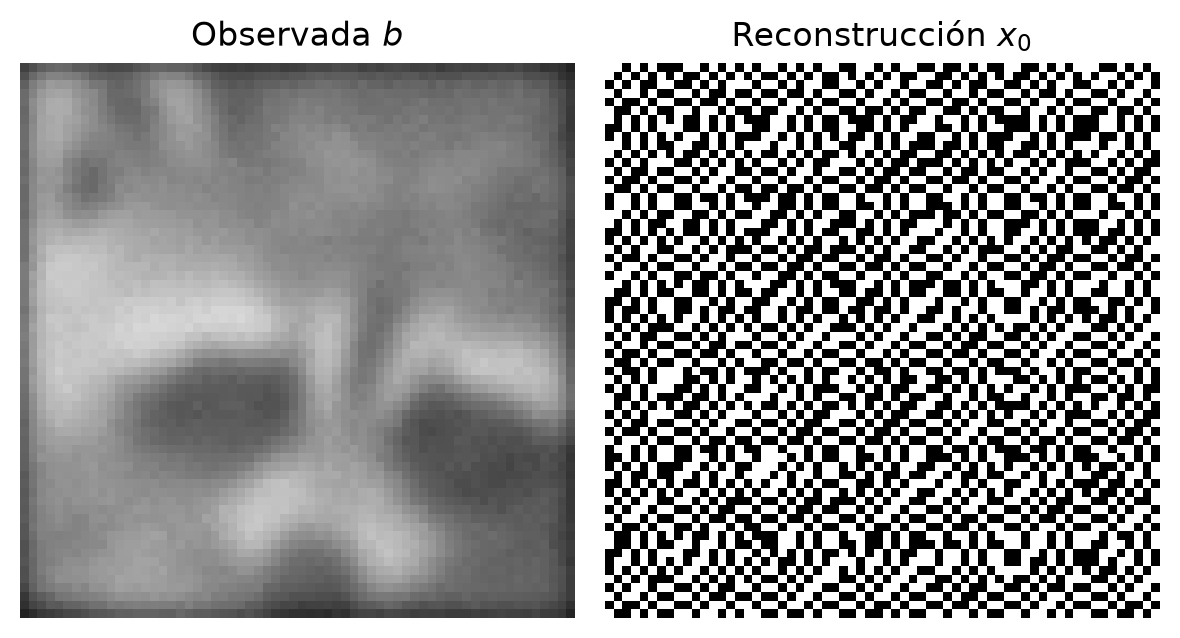
\includegraphics[width=6cm]{reconstruccion_b.png}
    \caption{Comparación imagen Observada b y Reconstrucción \(x_0\)}
    \label{fig:comparación_1}
  \end{figure}

  \subsection*{• Respuestas}

  Resultados Numéricos:

  - Norma: \(\|x_0\|_2=3.503\cdot10^5\)

  - Máximo Absoluto: \(\max_i|x_{0,i}|=1.871\cdot10^4\)

  - Residuo: \(\|Ax_0-b\|_2=5.626\cdot10^{-12}\)

  \smallskip

  Al comparar las imágenes, se observa claramente que la imagen \(x_0\) no se parece a la imagen observada \(b\). Si bien esta última se encuentra desenfocada, todavía es posible distinguir las características y el rostro de lo que parece ser un mapache. En cambio, en \(x_0\) se pueden observar píxeles blancos y negros que impiden identificar alguna figura reconocible.

  Esta distorsión se puede entender a partir de los resultados numéricos obtenidos. En primer lugar, la norma de la reconstrucción es \(\|x_0\|_2=3.503\cdot10^5\). Sabiendo que la norma máxima de una imagen válida es de \(64\), podemos notar cómo la norma obtenida es considerablemente mayor a la esperada, lo que provoca que su magnitud sea desproporcionada y dificulte la interpretación de los píxeles obtenidos.

  Por otro lado, se obtuvo que el máximo absoluto de sus componentes es \(\max_i|x_{0,i}|=1.871\cdot10^4\). Esta cifra es significantivamente superior, considerando la intensidad de cada píxel debería pertener al intervalo \([0,1]\). Al no respetarse estos límites, los píxeles se saturan creando contrastes extremos de blanco y negro que arruinan la imagen reconstruida.

  Finalmente, el residuo obtenido es \(\|Ax_0-b\|_2=5.626\cdot10^{-12}\), un valor que es prácticamente cero. Gracias a este resultado sabemos que \(x_0\) satisface el sistema \(Ax=b\). Sin embargo, esto no garantiza que la solución obtenida tenga sentido como imagen.

  En conclusión, aunque \(x_0\) satisface el sistema, sus valores no cumplen las condiciones esperadas para una imagen válida, lo que concuerda con la distorsión que se observa en la reconstrucción.

  \item \textbf{Explicación.}

  Sabemos que $x_0$ es la solución calculada mediante mínimos cuadrados (o directamente resolviendo el sistema), por lo que satisface $A x_0 = b$. Además, la observación real está dada por $b = A x^* + \eta$, donde $x^*$ es la imagen verdadera y $\eta$ es el ruido.

  Igualando ambas expresiones para $b$:
  \begin{align*}
  A x_0 &= A x^* + \eta \\
  A x_0 -A x^* &= \eta\\
  A(x_0 - x^*) &= \eta
  \end{align*}

  Multiplicamos a la izquierda por $A^T$:
  \begin{equation*}
  A^T A(x_0 - x^*) = A^T \eta
  \end{equation*}

  Calculamos el producto interno de ambos lados con el vector propio $v_i$:
  \begin{equation*}
  \langle A^T A(x_0 - x^*), v_i \rangle = \langle A^T \eta, v_i \rangle
  \end{equation*}

  Utilizando la propiedad fundamental del producto interno y la matriz transpuesta ($\langle M u, v \rangle = \langle u, M^T v \rangle$), reescribimos:
  \begin{equation*}
  \langle x_0 - x^*, A^T A v_i \rangle = \langle \eta, A v_i \rangle
  \end{equation*}

  Dado que $v_i$ es un vector propio de $A^T A$ asociado al valor propio $\mu_i$, se cumple que $A^T A v_i = \mu_i v_i$. Sustituyendo esto en la ecuación:
  \begin{equation*}
  \langle x_0 - x^*, \mu_i v_i \rangle = \langle A v_i, \eta \rangle
  \end{equation*}

  Como $\mu_i$ es un escalar, sale del producto interno. Finalmente, despejamos:
  \begin{equation*}
  \mu_i \langle x_0 - x^*, v_i \rangle = \langle A v_i, \eta \rangle \quad \implies \quad \langle x_0 - x^*, v_i \rangle = \frac{\langle A v_i, \eta \rangle}{\mu_i}
  \end{equation*}

  \subsection*{Demostración de la cota del error (desigualdad)}

  Tomamos el valor absoluto a la igualdad demostrada en el paso anterior:
  \begin{equation*}
  |\langle x_0 - x^*, v_i \rangle| = \frac{|\langle A v_i, \eta \rangle|}{\mu_i}
  \end{equation*}

  Aplicamos la desigualdad de Cauchy-Schwarz ($|\langle u, v \rangle| \leq \|u\|_2 \|v\|_2$) en el numerador:
  \begin{equation*}
  |\langle A v_i, \eta \rangle| \leq \|A v_i\|_2 \|\eta\|_2
  \end{equation*}

  Para encontrar el valor de $\|A v_i\|_2$, lo elevamos al cuadrado y usamos propiedades del producto interno:
  \begin{equation*}
  \|A v_i\|_2^2 = \langle A v_i, A v_i \rangle = \langle v_i, A^T A v_i \rangle = \langle v_i, \mu_i v_i \rangle = \mu_i \|v_i\|_2^2
  \end{equation*}

  Dado que la base de vectores propios es ortonormal, sabemos que $\|v_i\|_2 = 1$. Por lo tanto, $\|A v_i\|_2^2 = \mu_i$, lo que implica que $\|A v_i\|_2 = \sqrt{\mu_i}$.

  Reemplazando esto en la desigualdad de Cauchy-Schwarz obtenida:
  \begin{equation*}
  |\langle x_0 - x^*, v_i \rangle| \leq \frac{\sqrt{\mu_i} \|\eta\|_2}{\mu_i} = \frac{\|\eta\|_2}{\sqrt{\mu_i}}
  \end{equation*}

  \subsection*{Explicación cualitativa del fallo en la reconstrucción}

  El término $\langle x_0 - x^*, v_i \rangle$ representa la magnitud del error de nuestra reconstrucción $x_0$ con respecto a la imagen original $x^*$ en la dirección del vector $v_i$. Como hemos demostrado, este error es inversamente proporcional a $\sqrt{\mu_i}$.

  El problema radica en que el sistema está sumamente mal condicionado. Se nos indica que existen muchos valores de $\mu_i < 10^{-6}$ y que el mínimo es $\mu_{min} \approx 2 \times 10^{-16}$. 

  Al intentar recuperar la imagen directamente (sin regularización), el ruido $\eta$ se divide por estos valores propios minúsculos. Por ejemplo, dividir por $\sqrt{\mu_{min}}$ equivale a multiplicar el ruido por $\approx 10^8$. Incluso si el ruido inicial es pequeño ($\|\eta\|_2 \approx 0.64$), la amplificación en las direcciones asociadas a valores propios pequeños es astronómica. 

  Dado que los verdaderos píxeles de la imagen pertenecen al intervalo $[0, 1]$, sumarles un error del orden de miles o millones destruye completamente la señal original. Esto explica por qué $x_0$ no se parece a una imagen, teniendo valores máximos irreales y una norma desproporcionadamente alta en lugar de la imagen original.

  \end{enumerate}
\despueslista

\seccion{(c) Regularización de Tikhonov}

\begin{enumerate}[label=\roman*., widest=iv]

  \item \textbf{Gradiente, Hessiana y único minimizador global.}

  Para \(\lambda > 0\) consideramos la función:

  \[
  J_\lambda(x)=\|Ax-b\|_2^2+\lambda\|x\|_2^2
  \]

  \subsubsection*{• Cálculo del gradiente}

  Para calcular el gradiente, necesitamos derivar cada término de la función respecto del vector \(x\). En primer lugar, podemos notar que el primer término de \(J_\lambda(x)\) corresponde a la función \(J_0(x)\) analizada en la parte (a). Por lo tanto, sabemos que:

  \[
  J_0(x)=\|Ax-b\|_2^2
  \implies
  \nabla J_0(x)=2A^T(Ax-b)
  \]

  Para el segundo término de la función, utilizamos la propiedad de la norma euclidiana al cuadrado (\(\|x\|_2^2=x^Tx\)) para reescribirlo y facilitar el cálculo de su gradiente:

  \[
  \lambda\|x\|_2^2=\lambda x^Tx
  \]

  Como \(\lambda\) es una constante, al derivar respecto de \(x\) obtenemos:

  \[
  \nabla(\lambda x^Tx)=2\lambda x
  \]

  Sumando los gradientes de cada término, obtenemos que el gradiente de \(J_\lambda\) es:

  \[
  \boxed{\nabla J_\lambda(x)=2A^T(Ax-b)+2\lambda x}
  \]

  \subsubsection*{• Cálculo de la Matriz Hessiana}

  Para calcular la matriz Hessiana, debemos encontrar las segundas derivadas parciales de una función. En este caso, \(J_\lambda\) depende del vector \(x\), podemos obtener la Hessiana derivando el gradiente respecto de \(x\), considerando que las matrices \(A\) y \(A^T\), el vector \(b\) y el parámetro \(\lambda\) son constantes.

  Como la derivada de \(2A^T(Ax-b)\) es \(2A^TA\) y la derivada de \(2\lambda x\) es \(2\lambda I\), la matriz Hessiana es:

  \[
  \boxed{H_{J_\lambda}=2A^TA+2\lambda I}
  \]

  \subsubsection*{• Valores propios de \(H_{J_\lambda}\)}

  Para demostrar que todos los valores propios de \(H_{J_\lambda}\) son mayores o iguales que \(2\lambda\), analizaremos cómo actúan los vectores propios de la Hessiana. Dado que \(H_{J_\lambda}=2(A^TA+\lambda I)\), y considerando que sumar un múltiplo de la matriz identidad no altera los vectores propios de una matriz, podemos usar directamente los vectores propios de \(A^TA\).

  Para ello, consideraremos que los vectores propios de \(A^TA\) cumplen con la propiedad \((A^TA)v_i=\mu_i v_i\), donde \(v_i\) es un vector propio no nulo y \(\mu_i\) su valor propio asociado. A partir de esta propiedad, evaluamos la Hessiana y obtenemos que:

  \[
  \begin{aligned}
  H_{J_\lambda}v_i
  &=2(A^TA+\lambda I)v_i\\
  &=2(A^TAv_i+\lambda v_i)\\
  &=2(\mu_i v_i+\lambda v_i)\\
  &=2(\mu_i+\lambda)v_i
  \end{aligned}
  \]

  Con este resultado, confirmamos que \(v_i\) también es un vector propio de \(H_{J_\lambda}\) y que su valor propio asociado es \(2(\mu_i+\lambda)\).

  Como en el ítem (a).ii se demostró que \(A^TA\) es una matriz semidefinida positiva, sabemos que sus valores propios cumplen con \(\mu_i\geq0\). Además, considerando que por enunciado sabemos que \(\lambda>0\), concluimos que:

  \[
  \boxed{2(\mu_i+\lambda)\geq2\lambda}
  \]

  De esta manera, queda demostrado que todos los valores propios de la matriz \(H_{J_\lambda}\) son mayores o iguales que \(2\lambda\).

  \subsubsection*{• Unicidad y existencia del minimizador global}

  Para demostrar que la función \(J_\lambda(x)\) tiene un único minimizador global, partiremos de que \(H_{J_\lambda}\) es definida positiva ya que todos sus valores propios son estrictamente positivos. Esto implica que la función es estrictamente convexa, lo que nos permite asegurar que, de existir un punto crítico, este será único y corresponderá al mínimo global.

  Para encontrar este punto, igualaremos el gradiente calculado en un inicio a cero:

  \[
  \nabla J_\lambda(x)=2A^T(Ax-b)+2\lambda x=0
  \]

  Simplificamos dividiendo por \(2\) y reordenamos términos:

  \[
  \begin{aligned}
  A^T(Ax-b)+\lambda x&=0\\
  A^TAx-A^Tb+\lambda x&=0\\
  A^TAx+\lambda x&=A^Tb\\
  (A^TA+\lambda I)x&=A^Tb
  \end{aligned}
  \]

  Como los valores propios de \((A^TA+\lambda I)\) son estrictamente positivos, la matriz es invertible. Al multiplicar por su inversa, despejamos la solución única:

  \[
  \boxed{x_\lambda=(A^TA+\lambda I)^{-1}A^Tb}
  \]

  Con esto se concluye que \(J_\lambda(x)\) tiene un único minimizador global, y es \(x_\lambda\).

  \bigskip

  \item \textbf{Descomposición de $\ip{x_\lambda}{v_i}$ y cota del aporte del ruido.}

  \subsubsection*{• Descomposición de $\ip{x_\lambda}{v_i}$}

  Para realizar la primera demostración, partiremos de la ecuación obtenida en el ítem (c).i:

  \[
  x_\lambda=(A^TA+\lambda I)^{-1}A^Tb
  \]

  Como sabemos que \(b=Ax^\star+\eta\), sustituimos esta expresión en la fórmula de \(x_\lambda\):

  \[
  \begin{aligned}
  x_\lambda&=(A^TA+\lambda I)^{-1}A^T(Ax^\star+\eta)\\
  &=(A^TA+\lambda I)^{-1}A^TAx^\star+(A^TA+\lambda I)^{-1}A^T\eta
  \end{aligned}
  \]

  A continuación, calcularemos el producto interno de \(\langle x_\lambda,v_i\rangle\). Para esto, reemplazamos la expresión de \(x_\lambda\) y distribuimos la suma por linealidad (\(\langle a+b,c\rangle=\langle a,c\rangle+\langle b,c\rangle\)):

  \[
  \begin{aligned}
  \langle x_\lambda,v_i\rangle
  &=\left\langle (A^TA+\lambda I)^{-1}A^TAx^\star+(A^TA+\lambda I)^{-1}A^T\eta,v_i\right\rangle\\
  &=\left\langle (A^TA+\lambda I)^{-1}A^TAx^\star,v_i\right\rangle+\left\langle (A^TA+\lambda I)^{-1}A^T\eta,v_i\right\rangle
  \end{aligned}
  \]

  Luego, trasladamos la matriz al segundo argumento mediante la propiedad \(\langle Mu, v \rangle = \langle u, M^T v \rangle\). Como \((A^T A + \lambda I)^{-1}\) es simétrica, su tranpuesta es igual a si misma:

  \[
  \begin{aligned}
  \langle x_\lambda,v_i\rangle
  &=\left\langle A^TAx^\star,(A^TA+\lambda I)^{-1}v_i\right\rangle+\left\langle A^T\eta,(A^TA+\lambda I)^{-1}v_i\right\rangle
  \end{aligned}
  \]

  Como \(v_i\) es un vector propio de \(A^TA\), tal que \(A^TAv_i=\mu_i v_i\). Al sumar \(\lambda I\), obtenemos:

  \[
  \begin{aligned}
  (A^TA+\lambda I)v_i
  &=A^TAv_i+\lambda Iv_i\\
  &=\mu_i v_i+\lambda v_i\\
  &=(\mu_i+\lambda)v_i
  \end{aligned}
  \]

  \bigskip

  Como \(\mu_i+\lambda>0\), podemos multiplicar por la inversa y despejar:

  \[
  (A^TA+\lambda I)^{-1}v_i=\frac{1}{\mu_i+\lambda}v_i
  \]

  Reemplazamos esta expresión en los productos internos:

  \[
  \begin{aligned}
  \langle x_\lambda,v_i\rangle
  &=\left\langle A^TAx^\star,\frac{1}{\mu_i+\lambda}v_i\right\rangle+\left\langle A^T\eta,\frac{1}{\mu_i+\lambda}v_i\right\rangle
  \end{aligned}
  \]

  Aplicando la propiedad \(\langle a,cv\rangle=c\langle a,v\rangle\), sacamos los escalares de los productos internos y volviendo a utilizar \(\langle Mu,v\rangle=\langle u,M^Tv\rangle\) para trasladar las matrices restantes (teniendo en cuenta que, \(A^TA\) es simétrica, y que la transpuesta de \(A^T\) es \(A\)), obtenemos:

  \[
  \begin{aligned}
  \langle x_\lambda,v_i\rangle
  &=\frac{1}{\mu_i+\lambda}\langle x^\star,A^TAv_i\rangle+\frac{1}{\mu_i+\lambda}\langle\eta,Av_i\rangle
  \end{aligned}
  \]

  Por último, reemplazamos \(A^TAv_i=\mu_i v_i\), sacamos el escalar \(\mu_i\) y aplicamos la propiedad de simetría del producto interno \(\langle a,b\rangle=\langle b,a\rangle\):

  \[
  \begin{aligned}
  \langle x_\lambda,v_i\rangle
  &=\frac{1}{\mu_i+\lambda}\langle x^\star,\mu_i v_i\rangle+\frac{\langle Av_i,\eta\rangle}{\mu_i+\lambda}\\
  &=\frac{\mu_i}{\mu_i+\lambda}\langle x^\star,v_i\rangle+\frac{\langle Av_i,\eta\rangle}{\mu_i+\lambda}
  \end{aligned}
  \]

  De esta manera, queda demostrado que:

  \[
  \boxed{
  \langle x_\lambda,v_i\rangle
  =
  \frac{\mu_i}{\mu_i+\lambda}\langle x^\star,v_i\rangle
  +
  \frac{\langle Av_i,\eta\rangle}{\mu_i+\lambda}
  }
  \]

  \subsubsection*{• Cota aporte de ruido}

  Para realizar la segunda demostración, partiremos del término asociado al ruido obtenido en la primera igualdad:

  \[
  \left|\frac{\langle Av_i,\eta\rangle}{\mu_i+\lambda}\right|
  \]

  Utilizaremos la desigualdad de Cauchy-Schwarz, que establece que \(|\langle u,v\rangle|\leq\|u\|_2\|v\|_2\). Aplicando esta propiedad al producto interno \(\langle Av_i,\eta\rangle\), obtenemos:

  \[
  \begin{aligned}
  \left|\frac{\langle Av_i,\eta\rangle}{\mu_i+\lambda}\right|
  =\frac{|\langle Av_i,\eta\rangle|}{\mu_i+\lambda}\
  \leq\frac{\|Av_i\|_2\|\eta\|_2}{\mu_i+\lambda}
  \end{aligned}
  \]

  Para calcular la norma de \(Av_i\), partiremos de su cuadrado (\(\|u\|_2^2=u^Tu\)), y aplicaremos la relación del vector propio \(A^TAv_i=\mu_i v_i\):

  \[
  \begin{aligned}
  \|Av_i\|_2^2
  &=(Av_i)^T(Av_i)\\
  &=v_i^TA^TAv_i\\
  &=v_i^T(\mu_i v_i)\\
  &=\mu_i v_i^Tv_i
  \end{aligned}
  \]

  Como los vectores propios \(v_i\) son unitarios, sabemos que \(v_i^Tv_i=\|v_i\|_2^2=1\). Por lo tanto:

  \[
  \|Av_i\|_2=\sqrt{\mu_i}
  \]

  Reemplazando este resultado en la desigualdad anterior, obtenemos:

  \[
  \left|\frac{\langle Av_i,\eta\rangle}{\mu_i+\lambda}\right|
  \leq\frac{\sqrt{\mu_i}\|\eta\|_2}{\mu_i+\lambda}
  \]

  Ahora aplicando la desigualdad \(\mu_i+\lambda\geq 2\sqrt{\mu_i\lambda}\) para acotar el denominador:

  \[
  \begin{aligned}
  \frac{\sqrt{\mu_i}}{\mu_i+\lambda}
  \leq\frac{\sqrt{\mu_i}}{2\sqrt{\mu_i\lambda}}\
  =\frac{1}{2\sqrt{\lambda}}
  \end{aligned}
  \]

  Por lo tanto, sustituyendo esto en la expresión anterior, queda demostrado que:

  \[
  \boxed{
  \left|\frac{\langle Av_i,\eta\rangle}{\mu_i+\lambda}\right|
  \leq\frac{\|\eta\|_2}{2\sqrt{\lambda}}
  }
  \]

  Esta cota depende únicamente de la norma del ruido y del parámetro \(\lambda\), por lo que se mantiene válida sin importar qué tan pequeño sea \(\mu_i\).

  \item \textbf{Interpretación.}

A partir de la ecuación demostrada en el inciso anterior:
\begin{equation*}
    \langle x_\lambda, v_i \rangle = \frac{\mu_i}{\mu_i + \lambda} \langle x^*, v_i \rangle + \frac{\langle A v_i, \eta \rangle}{\mu_i + \lambda}
\end{equation*}
Podemos interpretar el comportamiento de la reconstrucción dependiendo de la relación entre los valores propios $\mu_i$ y el parámetro de regularización $\lambda$:

\begin{itemize}

    \item \textbf{Caso $\mu_i \gg \lambda$:} En este caso, el factor $\frac{\mu_i}{\mu_i + \lambda} \approx 1$. Esto significa que la componente de la imagen verdadera $\langle x^*, v_i \rangle$ se recupera casi íntegramente. Como $\mu_i$ es grande, el término correspondiente al ruido se mantiene controlado y pequeño. Por lo tanto, en estas direcciones (que suelen contener la información estructural principal de la imagen), la señal se conserva.
    
    \item \textbf{Caso $\mu_i \ll \lambda$:} Aquí, el factor $\frac{\mu_i}{\mu_i + \lambda} \approx 0$. La componente de la imagen verdadera se suprime o atenúa fuertemente. Sin embargo, el término del ruido ahora queda dividido por un valor cercano a $\lambda$ en lugar del minúsculo $\mu_i$, por lo que el ruido está acotado por $\frac{\|\eta\|_2}{2\sqrt{\lambda}}$ y no explota. El método actúa como un filtro que sacrifica información en estas direcciones para evitar la amplificación catastrófica del ruido.
    
    \item \textbf{Si $\lambda$ es muy pequeño ($\lambda \to 0$):} La regularización pierde su efecto y el método se aproxima a la solución de mínimos cuadrados ordinarios ($x_0$). El ruido en las componentes con $\mu_i \approx 0$ se amplificará de manera descontrolada. Se espera obtener una imagen completamente destruida por el ruido, similar a lo observado en el inciso (b).
    
    \item \textbf{Si $\lambda$ es muy grande ($\lambda \to \infty$):} El denominador $\mu_i + \lambda$ estará dominado por $\lambda$ para todos los $\mu_i$. Esto fuerza a que $\frac{\mu_i}{\mu_i + \lambda} \to 0$ en todas las componentes, lo que significa que el término de penalización $\|x\|_2^2$ es tan restrictivo que suprime la imagen verdadera. Se espera obtener una imagen que tienda a cero (completamente negra o plana), perdiendo toda información útil.
    
\end{itemize}

  \item \textbf{Implementación.} Completen la tabla y comparen las reconstrucciones.

  \begin{table}[H]
    \centering
    \begin{tabular}{>{\filatabla}l c c}
      \toprule[0.8bp]
                           & $\norm{x}_2$ & $\norm{Ax - b}_2$ \\
      \midrule[0.4bp]
      $x_0$                 &3.503e+05        &5.626e-12                  \\
      $\lambda = 10^{-3.5}$ &37.06            &0.5617                  \\
      $\lambda = 10^{-2.5}$ &36.02            &0.6169                   \\
      $\lambda = 1$         &17.18            &17.85                  \\
      \bottomrule[0.8bp]
    \end{tabular}
    \caption{Norma y residuo de cada reconstrucción.}
    \label{tab:ridge}
  \end{table}

  \begin{figure}[H]
    \centering
    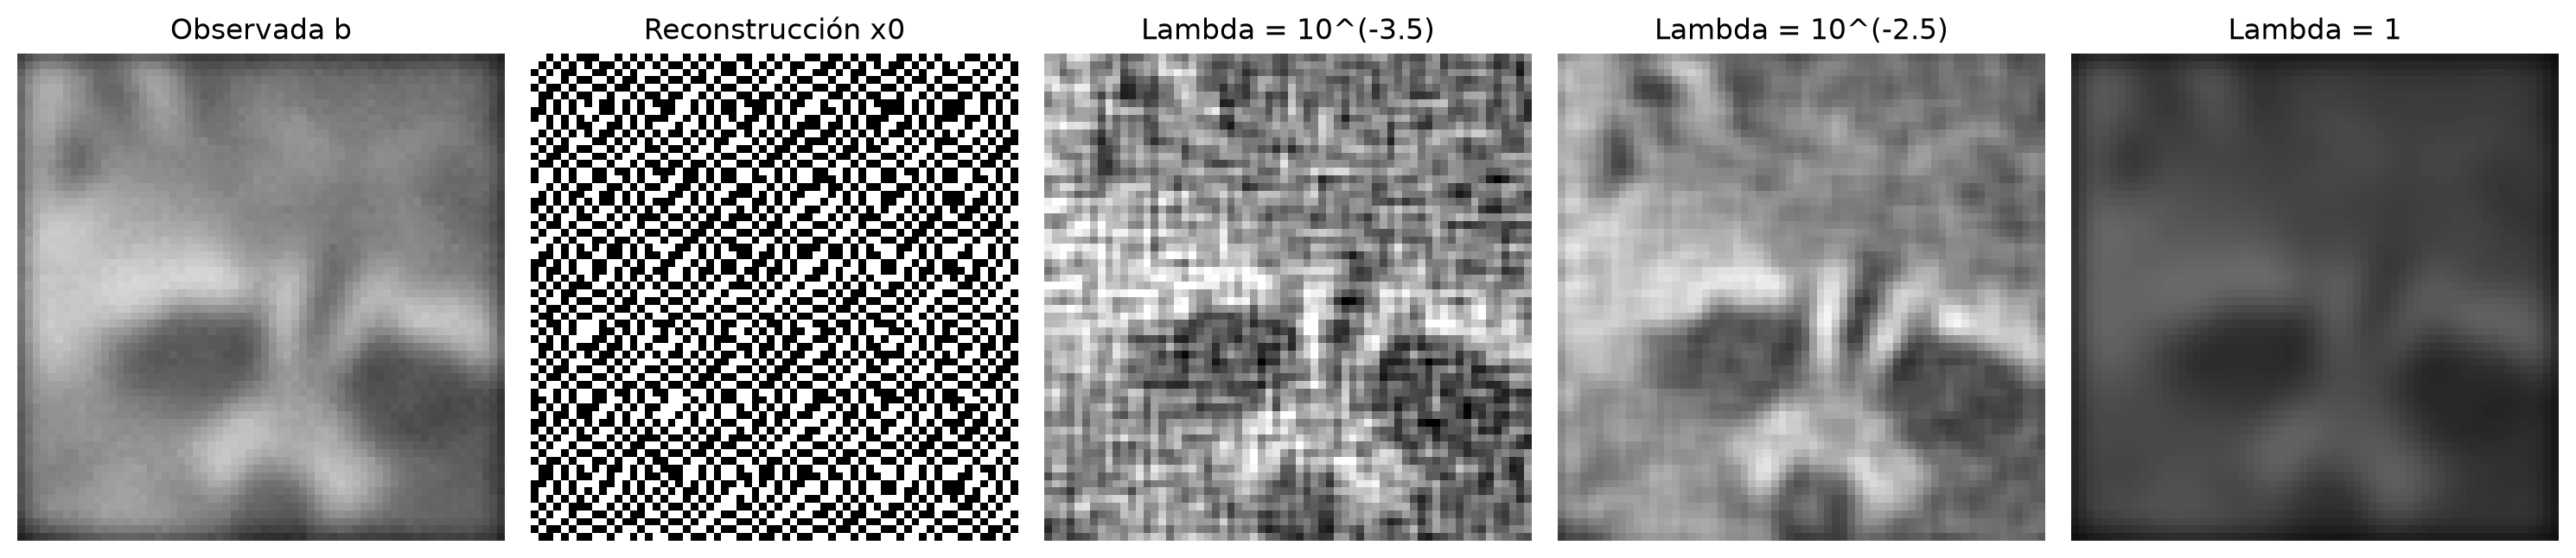
\includegraphics[width=15cm]{reconstrucciones_tikhonov.png}
    \caption{Comparación de reconstrucciones con distintos valores de \(\lambda\).}
    \label{fig:comparación_2}
  \end{figure}

  \subsubsection*{• Análisis de Imagenes y Conclusión}

  Analizando los resultados numéricos y las imagenes obtenidas, se concluye que \(\lambda = 10^{-2.5}\) entrega la mejor reconstrucción. Esto se debe a que permite distinguir con mayor claridad el rostro del mapache, presenta menos distorciones y tiene una norma de \(36.02\), inferior al máximo de \(64\). Además, su residuo de \(0.6169\) es el más cercano al nivel de ruido original \(\delta=0.64\), por lo que logra un mejor equilibrio entre reducir el ruido y conservar los detalles de la imagen en comparación con las otras reconstrucciones.
\end{enumerate}
\despueslista

\seccion{(d) Píxeles dañados}

  \begin{figure}[H]
    \centering
    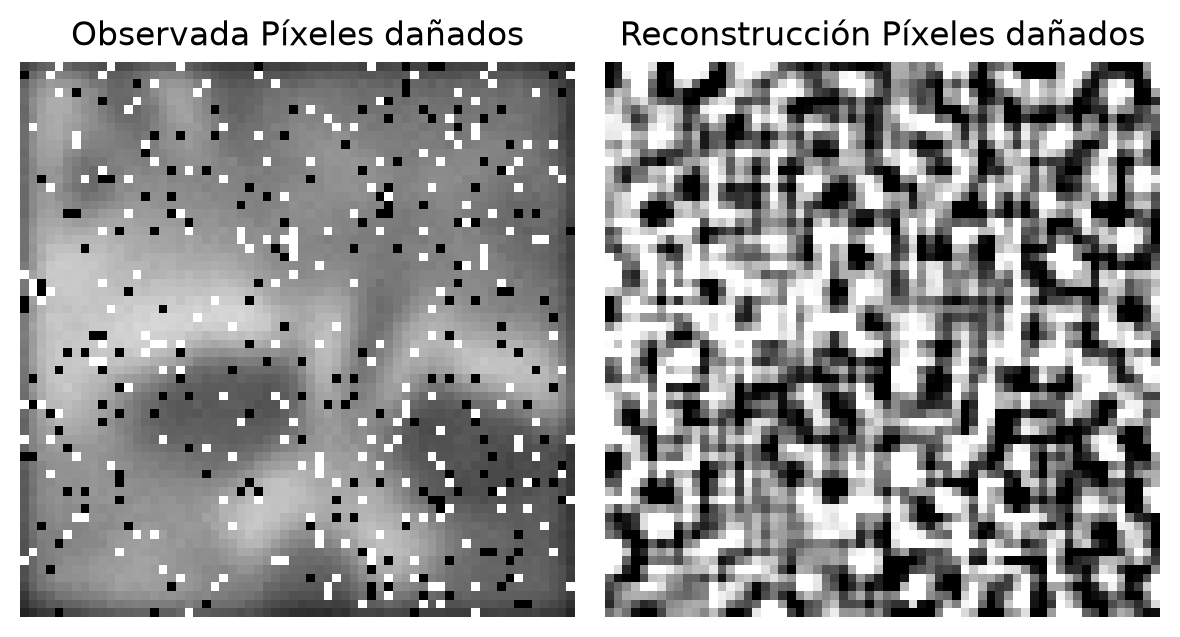
\includegraphics[width=8cm]{reconstruccion_danada.png}
    \caption{Comparación entre la imagen observada con píxeles dañados y su reconstrucción}
    \label{fig:comparación_3}
  \end{figure}

\begin{enumerate}[label=\roman*., widest=iii]
  \item \textbf{$\tilde{\eta} = \eta + (\tilde{b} - b)$ e interpretación de sus sumandos.}

  \subsubsection*{• Demostración $\tilde{\eta} = \eta + (\tilde{b} - b)$}

  Para demostrar que \(\eta=\eta+(\tilde b-b)\), partiremos de la definición para la observación con pixeles dañados \(\tilde b=Ax^\star+\tilde{\eta}\). Despejamos \(\tilde{\eta}\):

  \[
  \tilde{\eta}=\tilde b-Ax^\star
  \]

  Por otra parte, de la defición de la observación desenfocada obtenemos \(Ax^\star=b-\eta\). Reemplazamos esto en la ecuación de \(\tilde{\eta}\):

  \[
  \begin{aligned}
  \tilde{\eta}
  &=\tilde b-Ax^\star\\
  &=\tilde b-(b-\eta)\\
  &=\eta+(\tilde b-b)
  \end{aligned}
  \]

  De esta manera queda demostrado que:

  \[
  \boxed{\tilde{\eta}=\eta+(\tilde b-b)}
  \]

  \subsubsection*{• Interpretación de los sumandos}

  El ruido total de la observación defectuosa ($\tilde{\eta}$) está compuesto por la suma de dos efectos físicos distintos:

  1. \textbf{El sumando $\eta$ (Ruido natural del sensor):} Representa el ruido térmico/electrónico estándar presente en cualquier fotografía. Es un ruido de magnitud pequeña ($\|\eta\|_2 \approx 0.64$) y aleatorio.
  
  2. \textbf{El sumando $(\tilde{b} - b)$ (Corrupción por daño de hardware):} Representa exclusivamente el error masivo introducido por el $10\%$ de píxeles estropeados. Es un "ruido impulsivo" o determinista de magnitud altísima. Para los píxeles sanos, esta diferencia es cero, pero en los píxeles dañados (clavados en 0 o 1), la diferencia respecto a la observación sana $b$ es enorme, dominando por completo el valor del ruido total $\tilde{\eta}$. \\ 

  \item \textbf{$\norm{\tilde{b} - b}_2$ y comparación de $\norm{\tilde{\eta}}_2$ con $\delta$.}

  \subsubsection*{• Resultados numéricos}

  \(\|\tilde{b} - b\|_2\): 10.74

  Delta (\(\delta\)): 0.64s
  
  \subsubsection*{• Comparación}

  Para realizar la comparación, primero calcularemos \(\|\tilde{\eta}\|_2\). Como quedó demostrado en el ítem (d).i que \(\tilde{\eta}=\eta+(\tilde b-b)\), aplicamos la desigualdad triangular para obtener:

  \[
  \|\tilde{\eta}\|_2 = \|\eta + (\tilde{b} - b)\|_2 \le \|\eta\|_2 + \|\tilde{b} - b\|_2
  \]

  Sabemos que \(\|\eta\|_2 \approx \delta = 0.64\) y que \(\|\tilde{b} - b\|_2= 10.74\), reemplazamos los valores numéricos y obtenemos:

  \[
  \boxed{\|\tilde{\eta}\|_2 \le 0.64 + 10.74 = 11.38}
  \]

  Al comparar \(\norm{\tilde{\eta}}_2\) con el ruido original (\(\delta=0.64\)), podemos observar que el ruido total es considerablemente mayor debido a los píxeles dañados. Esto coincide con lo observado en la reconstrucción, donde el rostro del mapache deja de distinguirse y aparecen numerosas distorsiones. Por lo tanto, los resultados evidencian cómo las alteraciones adicionales en los datos pueden afectar la calidad de la imagen.

  \item \textbf{¿Por qué fracasa la reconstrucción? ¿Bastaría con aumentar $\lambda$?}\\

  \textbf{Razón del fracaso:}

  Sustituyendo $\eta$ por $\tilde{\eta}$ en la ecuación derivada en (c.ii), obtenemos:
  
\begin{equation*}
    \langle x_\lambda, v_i \rangle = \frac{\mu_i}{\mu_i + \lambda} \langle x^*, v_i \rangle + \frac{\langle A v_i, \tilde{\eta} \rangle}{\mu_i + \lambda}
\end{equation*}

  Como se calculó anteriormente, el ruido $\tilde{\eta}$ tiene una norma gigantesca dominada por los píxeles defectuosos ($\tilde{b} - b$). Esto provoca que el numerador del segundo sumando, $\langle A v_i, \tilde{\eta} \rangle$, alcance valores extremos. En consecuencia, el término de error eclipsa por completo a la componente de la imagen verdadera ($\frac{\mu_i}{\mu_i + \lambda} \langle x^*, v_i \rangle$), resultando en una reconstrucción fallida y completamente dominada por el ruido impulsivo.

\textbf{¿Bastaría con aumentar $\lambda$?} \\

  No, no bastaría. Para mitigar un ruido $\tilde{\eta}$ de tal magnitud, sería necesario aumentar $\lambda$ a un valor extremadamente grande. Sin embargo, recordando el análisis cualitativo del inciso (c.iii), si $\lambda$ es excesivamente grande, el denominador $\mu_i + \lambda$ domina para todos los valores propios $\mu_i$. 

  Esto fuerza a que el factor de recuperación de la señal $\frac{\mu_i}{\mu_i + \lambda}$ tienda a $0$. Al hacer esto, no solo suprimiríamos el ruido, sino que borraríamos por completo la imagen verdadera $x^*$. Pasaríamos de una reconstrucción ruidosa a una imagen completamente plana o negra, lo cual explica por qué la regularización de Tikhonov ($L_2$) no es robusta ante valores atípicos (outliers) severos como los píxeles dañados.

\end{enumerate}
\despueslista

% =====================================================================
\problema{Red neuronal con dos capas ocultas}
% =====================================================================

\seccion{(a) Derivada de la sigmoide}
\begin{enumerate}[label=\roman*]
  \item \textbf{construcción de $\sigma'$}
  
  considerando la funcion:
  \[\sigma(t)=\frac{1}{1+e^{-t}}\]
  notamos que podemos realizar una transformacion algebraica tal que
  \[\frac{1}{1+e^{-t}} = (1+e^{-t})^{-1}\]
  derivamos haciendo uso de la regla de la cadena:

  \[\sigma'(t)=-(1+e^{-t})^{-2}(-e^{-t}) = \frac{e^{-t}}{(1+e^{-t})^{2}}\]

  comprobamos si se satisface $\sigma'(t) = \sigma(t)(1 - \sigma(t))$

  \[
  \begin{aligned}
  \sigma(t)(1-\sigma(t))
  &= (\frac{1}{1+e^{-t}})(1 - \frac{1}{1+e^{-t}})\\
  &= \frac{1}{1+e^{-t}} - \frac{1}{(1+e^{-t})^2}\\
  &= \frac{1 + e^{-t} - 1}{(1+e^{-t})^2}\\
  &= \frac{e^{-t}}{(1+e^{-t})^2}\\
  &= \sigma'(t)
  \end{aligned}
  \]

  \bigskip\bigskip\bigskip\bigskip\bigskip\bigskip\bigskip\bigskip\bigskip\bigskip\bigskip\bigskip\bigskip
  
  \item \textbf{Deducción de intervalo}

  ya que $\forall t \in \mathbb{R}, \quad (e^{-t} > 0)$, deducimos que $0 < \sigma'(t)$\\
  Luego notamos que $\sigma(t)(1 - \sigma(t)) = (\sigma^2(t) - \sigma(t)) = (\sigma(t) - \frac{1}{2})^2 - \frac{1}{4}$\\
  ya que $\forall x \in \mathbb{R}, \quad x^2 \geq 0$, planteamos la siguiente desigualdad:


  \[
  \begin{aligned}
  (\sigma(t) - \frac{1}{2})^2 &\geq 0\\
  \Rightarrow \sigma^2(t) - \sigma(t) + \frac{1}{4} &\geq 0\\
  \Rightarrow \sigma(t) - \sigma^2(t) &\leq \frac{1}{4}\\
  \Rightarrow \sigma(t)(1-\sigma(t)) &\leq \frac{1}{4}\\
  \Rightarrow \sigma'(t) &\leq \frac{1}{4}
  \end{aligned}
  \]

  Por lo que se deduce que $0 < \sigma'(t) \leq \frac{1}{4}$.

  \item \textbf{Buscar el punto donde $\sigma'$ alcanza su máximo}
  
  Para encontrar el máximo de $\sigma'(t)$ podemos usar puntos críticos de $\sigma''(t)$.\\
  Por regla de la cadena tenemos que:

  \[
  \begin{aligned}
  \sigma''(t)
  &= \frac{-e^{-t}(1+e^{-t})^2 - 2(1+e^{-t})(-e^{-t})(e^{-t})}{(1+e^{-t})^4}\\
  &= \frac{-e^{-t}(1+e^{-t})-2(-e^{-t})(e^{-t})}{(1+e^{-t})^3}\\
  &= \frac{-e^{-t}-e^{-2t}+2e^{-2t}}{(1+e^{-t})^3}\\
  &= \frac{e^{-2t}-e^{-t}}{(1+e^{-t})^3}\\
  &= \frac{e^{-t}(e^{-t}-1)}{(1+e^{-t})^3}
  \end{aligned}
  \]

  Teniendo en cuenta que $\forall t \in \mathbb{R}, e^t \geq 0$\\
  Buscamos punto crítico:

  \[
  \frac{e^{-t}(e^{-t}-1)}{(1+e^{-t})^3} = 0
  \Rightarrow (e^{-t}-1) = 0
  \Rightarrow e^{-t} = 1
  \Rightarrow t = 0
  \]

  notamos que si $t > 0 \rightarrow \sigma''(t) < 0$ y si $t < 0 \rightarrow \sigma''(t) > 0$.\\ Por lo que $\sigma'(t)$ tiene un máximo en $t = 0$

  \[
  \sigma'(0) = \frac{e^{0}}{(1+e^{0})^{2}} = \frac{1}{4}
  \]
\end{enumerate}

\seccion{(b) Función de pérdida y su gradiente}

\begin{enumerate}[label=\roman*]

  \item \textbf{Definir objetos matematicos}

  \[z_{1,i} = a_1x_i+b1, \quad h_{1,i} = \sigma(z_1,i), \quad z_{2,i}=a_2h_{1,i}+b_2, \quad h_{2,i}=\sigma(z_{2,i}),\]

  \[\hat{y}_i=c+vh_{2,i}, \quad e_i=\hat{y}_i-y_i, \quad L_i = \frac{e^2_i}{2}\]

  \[
    \sigma'(t) = \sigma(t)(1- \sigma(t))
    \]

  \[
  \theta = (a_1, b_1, a_2, b_2, v, c)
  \]

  \item \textbf{Funcion pérdida}

  considerando la función
  \[J(\theta) = \frac{1}{2N}\sum_{i=1}^{N}(\hat{y}_i - y_i)^2\]

  notamos que con los objetos matematicos previamente definidos,\\
  esta se puede escribir de multiples formas, tal que:

  \[J(\theta) = \frac{1}{2N}\sum_{i=1}^{N}(e_i)^2 = \frac{1}{N}\sum_{i=1}^{N}Li\]

  esto nos facilitara el desarollo del calculo de las 6 derivadas parciales de $\nabla_\theta J(\theta)$

  \item \textbf{Calcular las 6 derivadas parciales}


  \begin{enumerate}[label=\arabic*.]
    \item derivada parcial respecto a $\alpha_1$
    
    $a_1 \longrightarrow z_{1,i} \longrightarrow h_{1,i}\longrightarrow z_{2,i} \longrightarrow h_{2,i}\longrightarrow \hat{y}_i \longrightarrow L_i$

    \[
    \begin{aligned}
    L_i &= \frac{1}{2}(c+v\sigma(a_2(\sigma(a_1x_i+b_1))+b_2)-y_i)^2\\
    &\quad\Rightarrow\quad
    \frac{\partial L_i}{\partial a_1}
    = (c+v\sigma(a_2(\sigma(a_1x_i+b_1))+b_2)-y_i)
    (a_2\cdot v \cdot \sigma'(z_{2,i}) \cdot \sigma'(z_{1,i}) \cdot x_i)\\
    &= (e_i \cdot a_2\cdot v \cdot \sigma'(z_{2,i}) \cdot \sigma'(z_{1,i}) \cdot x_i)\\
    &= (e_i \cdot a_2\cdot v \cdot h_{2,i}(1 - h_{2,i}) \cdot h_{1,i}(1-h_{1,i}) \cdot x_i)
    \end{aligned}
    \]

    \item derivada parcial respecto a $b_1$
    
    $b_1 \longrightarrow z_{1,i} \longrightarrow h_{1,i}\longrightarrow z_{2,i} \longrightarrow h_{2,i}\longrightarrow \hat{y}_i \longrightarrow L_i$

    \[
    \begin{aligned}
    L_i &= \frac{1}{2}(c+v\sigma(a_2(\sigma(a_1x_i+b_1))+b_2) -y_i)^2\\
    &\quad\Rightarrow\quad
    \frac{\partial L_i}{\partial b_1}
    = (c+v\sigma(a_2(\sigma(a_1x_i+b_1))+b_2) -y_i)
    (a_2\cdot v \cdot \sigma'(z_{2,i}) \cdot \sigma'(z_{1,i}))\\
    &= e_i \cdot a_2\cdot v \cdot \sigma'(z_{2,i}) \cdot \sigma'(z_{1,i})\\
    &= e_i \cdot a_2\cdot v \cdot h_{2,i}(1 - h_{2,i}) \cdot h_{1,i}(1-h_{1,i})
    \end{aligned}
    \]

    \item derivada parcial respecto a $\alpha_2$

    $a_2 \longrightarrow z_{2,i} \longrightarrow h_{2,i}\longrightarrow \hat{y}_i \longrightarrow L_i$

    \[
    \begin{aligned}
    L_i &= \frac{1}{2}(c+v\sigma(a_2h_{1,i}+b_2) -y_i)^2\\
    &\quad\Rightarrow\quad
    \frac{\partial L_i}{\partial a_2}
    = (c+v\sigma(a_2h_{1,i}+b_2) -y_i)
    (h_{1,i}\cdot v \cdot \sigma'(z_{2,i}))\\
    &= (e_i \cdot h_{1,i}\cdot v \cdot \sigma'(z_{2,i}))\\
    &= (e_i \cdot h_{1,i}\cdot v \cdot h_{2,i}(1-h_{2,i}))
    \end{aligned}
    \]

    \item derivada parcial respecto a $b_2$
    
    $b_2 \longrightarrow z_{2,i} \longrightarrow h_{2,i}\longrightarrow \hat{y}_i \longrightarrow L_i$

    \[
      \begin{aligned}
        L_i &= \frac{1}{2}(c+v\sigma(a_2h_{1,i}+b_2) -y_i)^2\\
        &\quad\Rightarrow\quad
        \frac{\partial L_i}{\partial b_2}
        = (c+v\sigma(a_2h_{1,i}+b_2)-y_i)
        (v \cdot \sigma'(z_{2,i}))\\
        &= (e_i\cdot v \cdot \sigma'(z_{2,i}))\\
        &= (e_i \cdot v \cdot h_{2,i}(1-h_{2,i}))
      \end{aligned}
      \]

    \item derivada parcial respecto a $v$

    $v \longrightarrow \hat{y}_i \longrightarrow L_i$

    \[
    L_i = \frac{1}{2}(c+v \cdot h_{2,i} - y_i)^2
    \quad\Rightarrow\quad
    \frac{\partial L_i}{\partial v}
    = ((c+v \cdot h_{2,i} - y_i)h_{2,i})
    \;=\;(e_i \cdot h_{2,i})
    \]

    \item derivada parcial respecto a $c$
    
    $c \longrightarrow \hat{y}_i \longrightarrow L_i$

    \[
      L_i = \frac{1}{2}(c+v \cdot h_{2,i} - y_i)^2
      \quad\Rightarrow\quad
      \frac{\partial L_i}{\partial c}
      = (c+v \cdot h_{2,i} - y_i)
      \;=\;(e_i)
      \]
  \end{enumerate}

  \item \textbf{Expresar $\nabla_\theta J(\theta)$}
  
  notamos que entre derivadas parciales existen factores repetidos,
  por lo que a continuación definimos estos para expresar el gradiente de forma completa
    
    \[
  \varphi_{2,i} = e_i \cdot v \cdot h_{2,i}(1-h_{2,i}) ,
  \quad
  \varphi_{1,i} = \varphi_{2,i} \cdot h_{1,i}(1-h_{1,i}) \cdot a_2
  \]

  ya con todo lo necesario, expresamos el gradiente de la siguiente forma:
  \[
  \nabla_\theta J(\theta) = \frac{1}{N}\sum_{i=1}^{N}
  \begin{pmatrix}
    \varphi_{1,i}x_i \\
    \varphi_{1,i} \\
    \varphi_{2,i}h_{1,i} \\
    \varphi_{2,i} \\
    e_ih_{2,i} \\
    e_i
    \end{pmatrix}
    \]

\end{enumerate}

  \seccion{(c) Implementación y verificación del gradiente}
  
  Reporten $\theta_0$, $J(\theta_0)$ y el error máximo $E$.
  
  Dado un $\theta$ arbitrario:\\
  $\theta_0 = (-0.28824117\quad -0.08699002\quad  -0.91449653\quad -0.6212921\quad   0.11734601\quad -0.07469821)$\\
  $J(\theta_0) = 0.7848795168338227$

  \begin{table}[H]
  \centering
  \begin{tabular}{>{\filatabla}c r r r}
    \toprule[0.8bp]
    Parámetro & Fórmula de (b) \quad\quad\quad\quad\quad & $D_j$\quad\quad\quad\quad\quad & Diferencia aproximada\\
    \midrule[0.4bp]
    $a_1$ & $\frac{J(a_1 + 10^{-5}, b_1, a_2, b_2, v, c) - J(a_1 - 10^{-5}, b_1, a_2, b_2, v, c)}{2 \cdot 10^5}$ & $-0.0026258517638044765$ & $2.67 \cdot 10^{-11}$\\
    $b_1$ & $\frac{J(a_1, b_1 + 10^{-5}, a_2, b_2, v, c) - J(a_1, b_1 - 10^{-5}, a_2, b_2, v, c)}{2 \cdot 10^5}$ & $0.004549815707521887$ & $5.44 \cdot 10^{-12}$\\
    $a_2$ & $\frac{J(a_1, b_1, a_2 + 10^{-5}, b_2, v, c) - J(a_1, b_1, a_2 - 10^{-5}, b_2, v, c)}{2 \cdot 10^5}$ & $-0.010386437077070099$ & $1.53 \cdot 10^{-11}$\\
    $b_2$ & $\frac{J(a_1, b_1, a_2, b_2 + 10^{-5}, v, c) - J(a_1, b_1, a_2, b_2 - 10^{-5}, v, c)}{2 \cdot 10^5}$ & $-0.019980829651933263$ & $1.61 \cdot 10^{-11}$\\
    $v$   & $\frac{J(a_1, b_1, a_2, b_2, v + 10^{-5}, c) - J(a_1, b_1, a_2, b_2, v - 10^{-5}, c)}{2 \cdot 10^5}$ & $-0.22715555679786445$ & $1.92 \cdot 10^{-11}$\\
    $c$   & $\frac{J(a_1, b_1, a_2, b_2, v, c + 10^{-5}) - J(a_1, b_1, a_2, b_2, v, c - 10^{-5})}{2 \cdot 10^5}$ & $-0.9073814595084161$ & $8.23 \cdot 10^{-12}$\\
    \bottomrule[0.8bp]
  \end{tabular}
  \caption{Gradiente en $\theta_0$: fórmulas de (b) y diferencias centradas.}
  \label{tab:gradiente}
\end{table}

  Notamos que, al utilizar $\theta_0$, el mayor error absoluto se presenta al calcular la diferencia correspondiente al parametro $a_1$, tal que:
\[E = |\frac{\partial J}{\partial a_1}\theta_0 - D_1| \approx 2.67 \cdot 10^{-11}\]

\seccion{(d) Descenso del gradiente}

\begin{figure}[htbp]
    \centering

    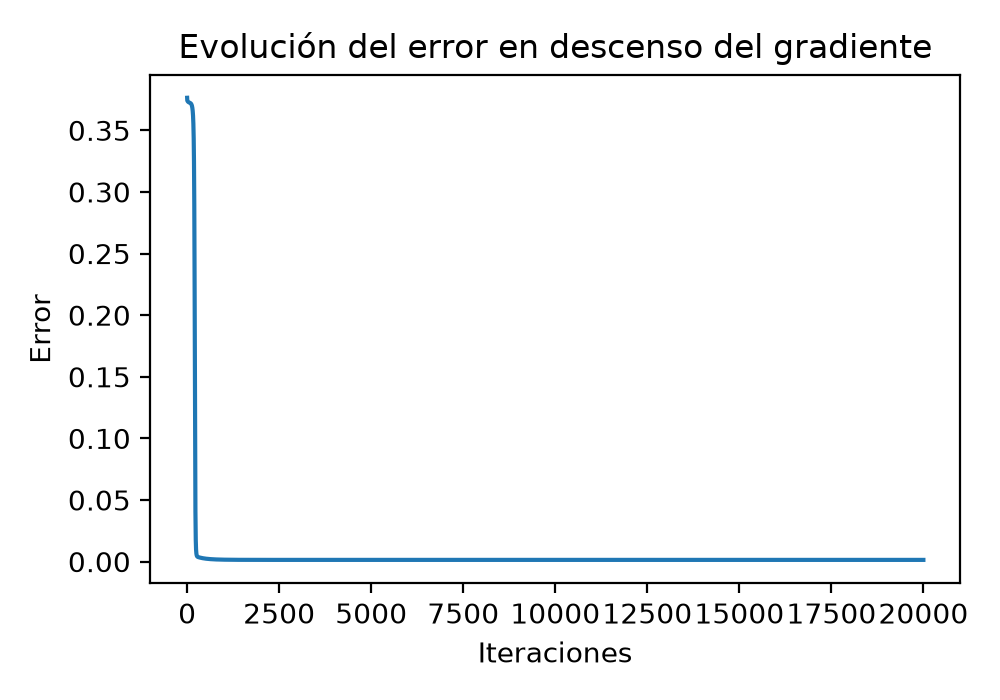
\includegraphics[width=0.48\textwidth]{figuras/figuras_p2/evo_des_gradiente.png}
    \hfill
    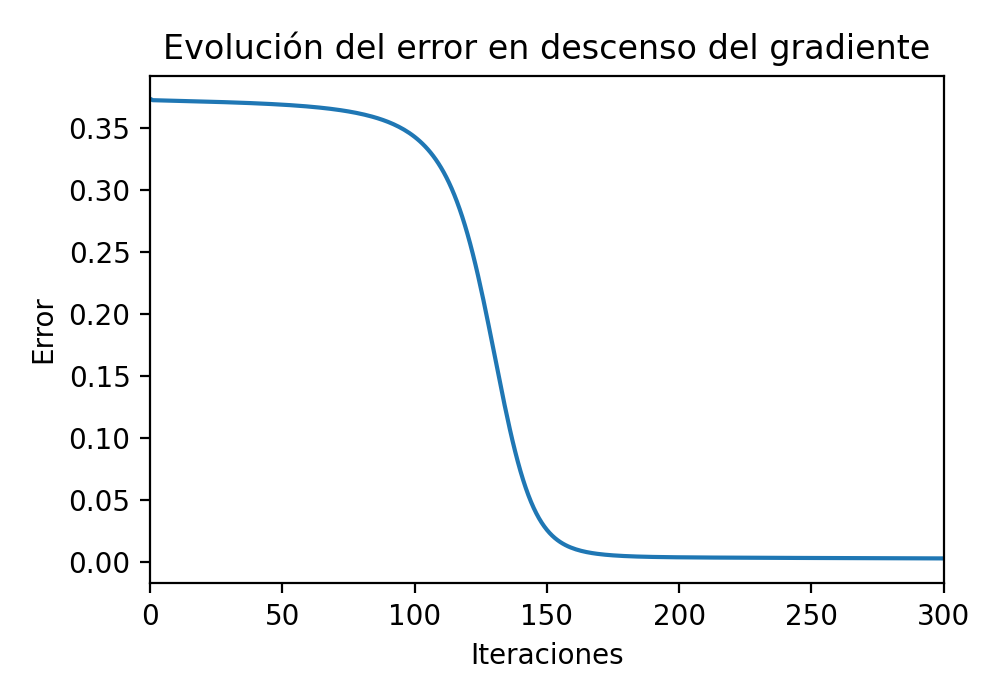
\includegraphics[width=0.48\textwidth]{figuras/figuras_p2/evo_des_gradiente_cambio.png}

    \caption{Evolución del error $J(\theta_k)$ en función de $k$.}
    \label{fig:evolucion_error}
\end{figure}


La grafica presenta un comportamiento decreciente no lineal, inicialmente el error disminuye de manera suave, luego aproximadamente en el rango de iteraciones [90, 160] la funcion desciende abruptamente, hasta que se estabiliza en un valor cercano a 0, indicando que esta ha llegado a un minimo, tal que el comportamiento del método de descenso gradiente converge rapidamiente a un minimo cercano a 0.

\bigskip\bigskip\bigskip\bigskip

\seccion{(e) Parámetros encontrados}

Los valores encontrados:\\
$\theta_{20000} \approx (4.8207018, 0.6801908, -4.0540688, 0.6141261, 3.5773664, -0.1000645)$\\
$J(\theta_{20000}) = 0.0013927707069917585$

\begin{figure}[h]
    \centering
    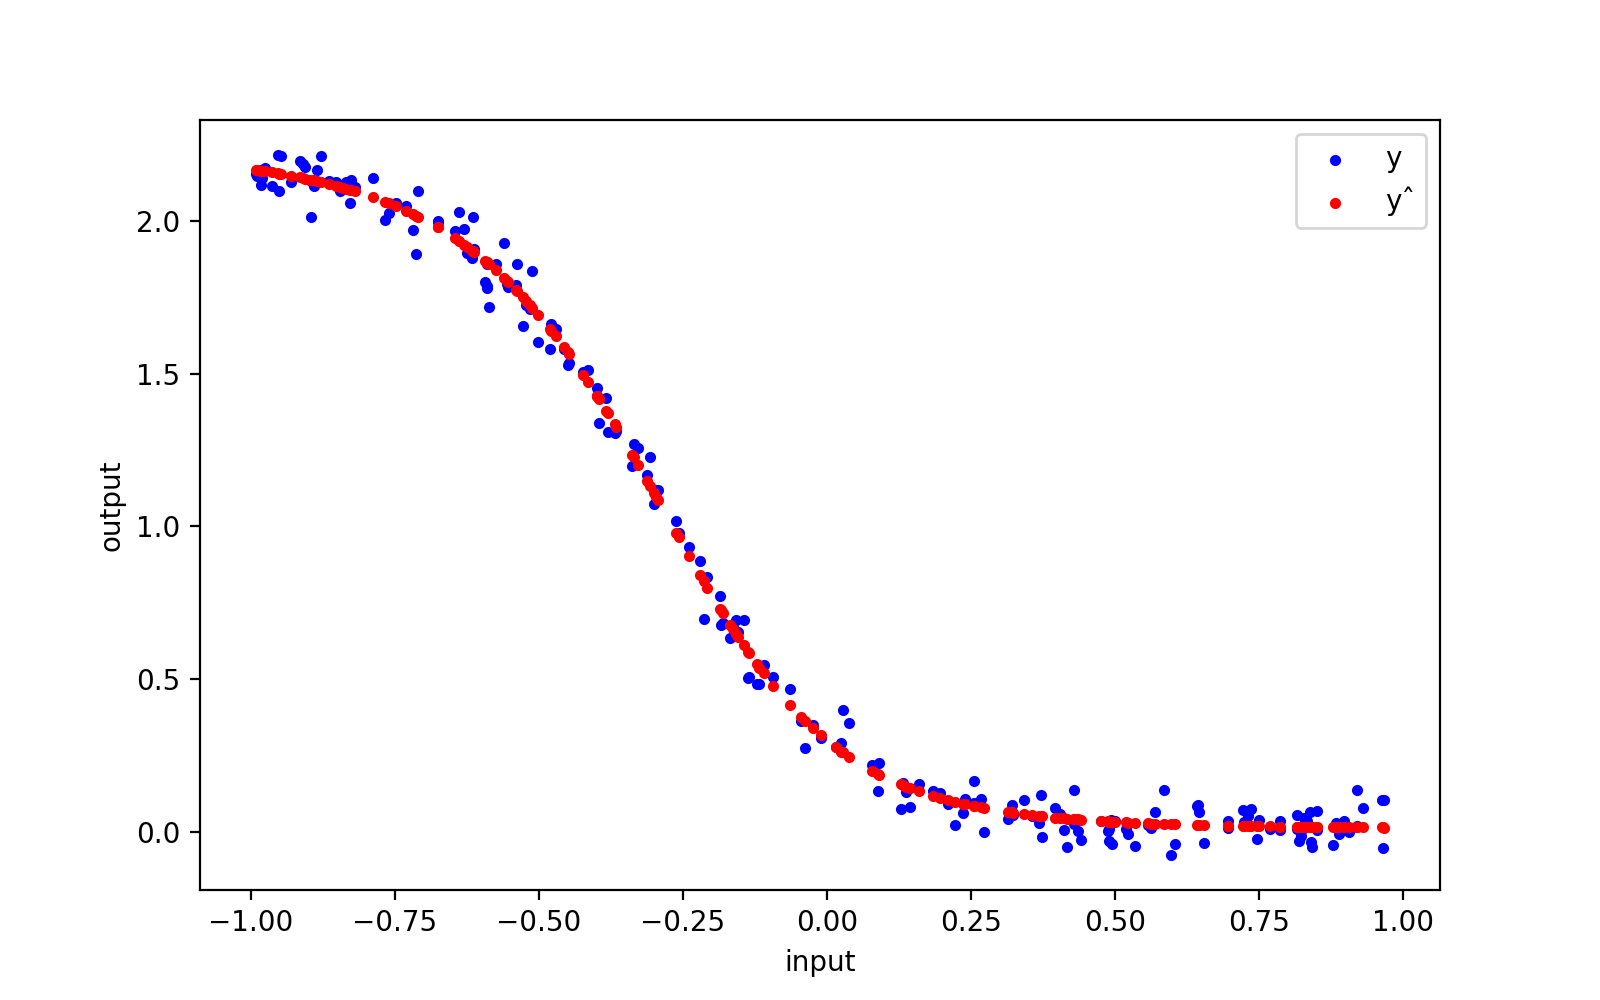
\includegraphics[width=0.5\textwidth]{figuras/figuras_p2/entrenamientoXcurva.png}
    \caption{entrenamiento y curva $x \mapsto \hat{y}(x;\theta_{20.000})$}
    \label{fig:entrenamientoXcurva}
\end{figure}
\newpage
\seccion{(f) Sensibilidad del entrenamiento}

\begin{enumerate}[label=\roman*., widest=ii]
  \item \textbf{Tamaño del paso.}

  Repetimos d), ahora para los $\alpha = 0.01, 0.1, 1, 2.5$ y observamos la gráfica de sus errores

  \begin{figure}[h]
    \centering
    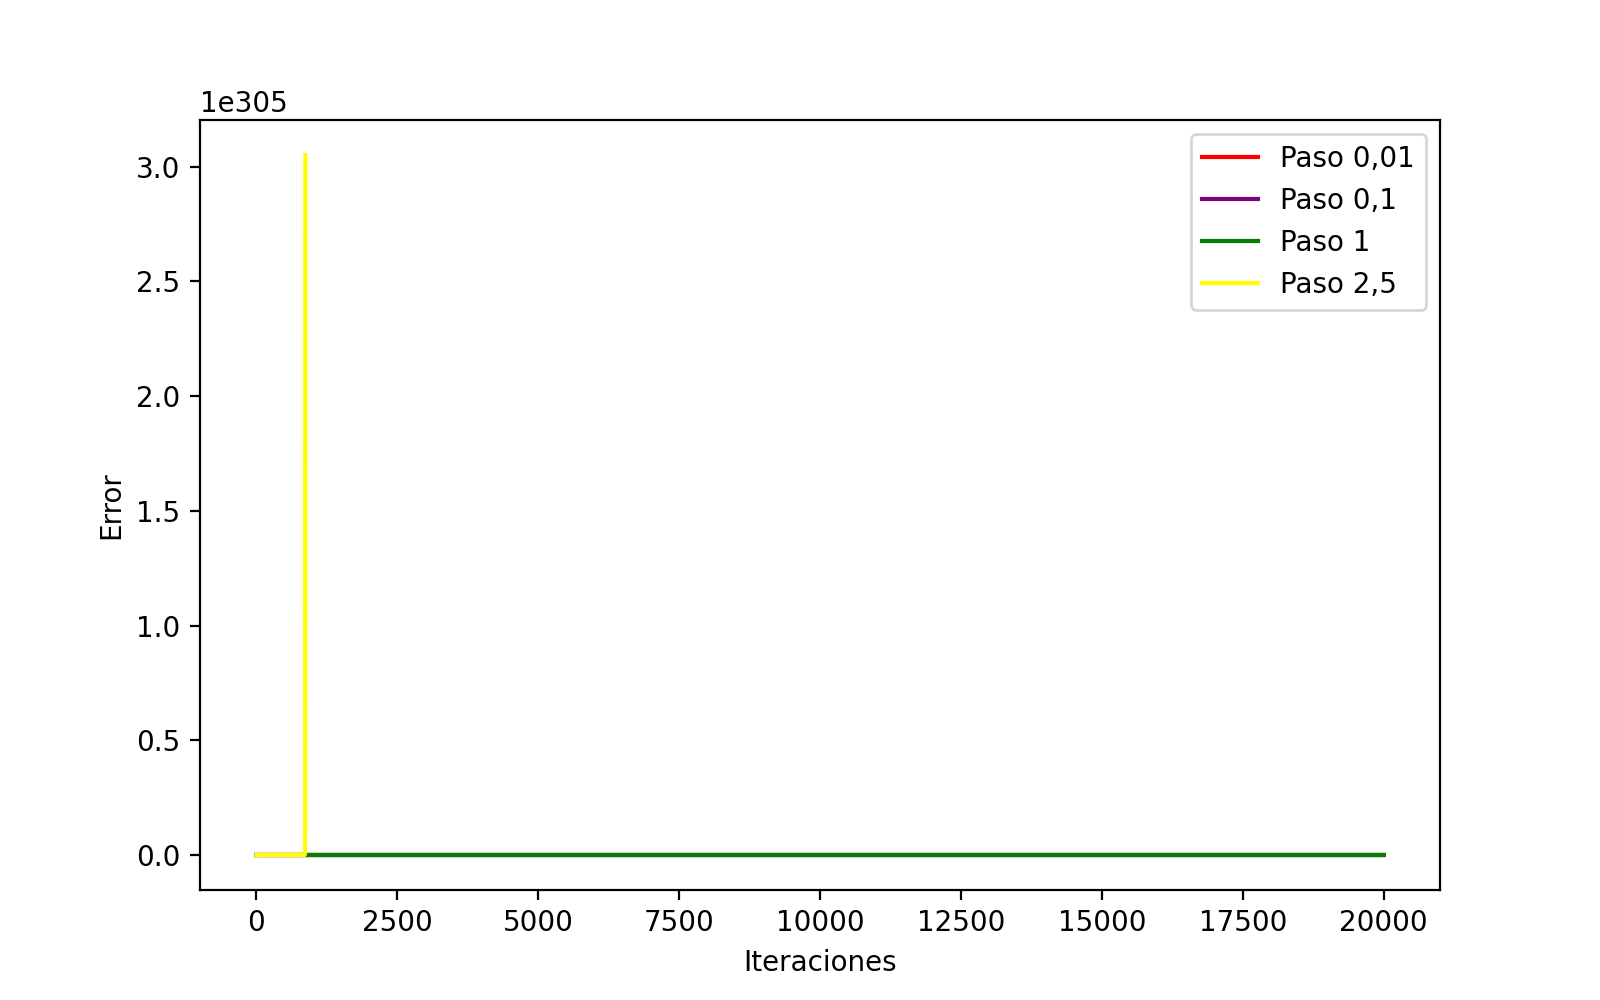
\includegraphics[width=0.5\textwidth]{figuras/figuras_p2/cuatro_curvas_error.png}
    \caption{Evolución errores de los 4 pasos}
    \label{fig:cuatro_error}
\end{figure}

  Dado que este gráfico no nos permite ver las curvas de cada paso, hacemos uno diferente para visualizar los pasos 0,01; 0,1 y 1

  \begin{figure}[h]
    \centering
    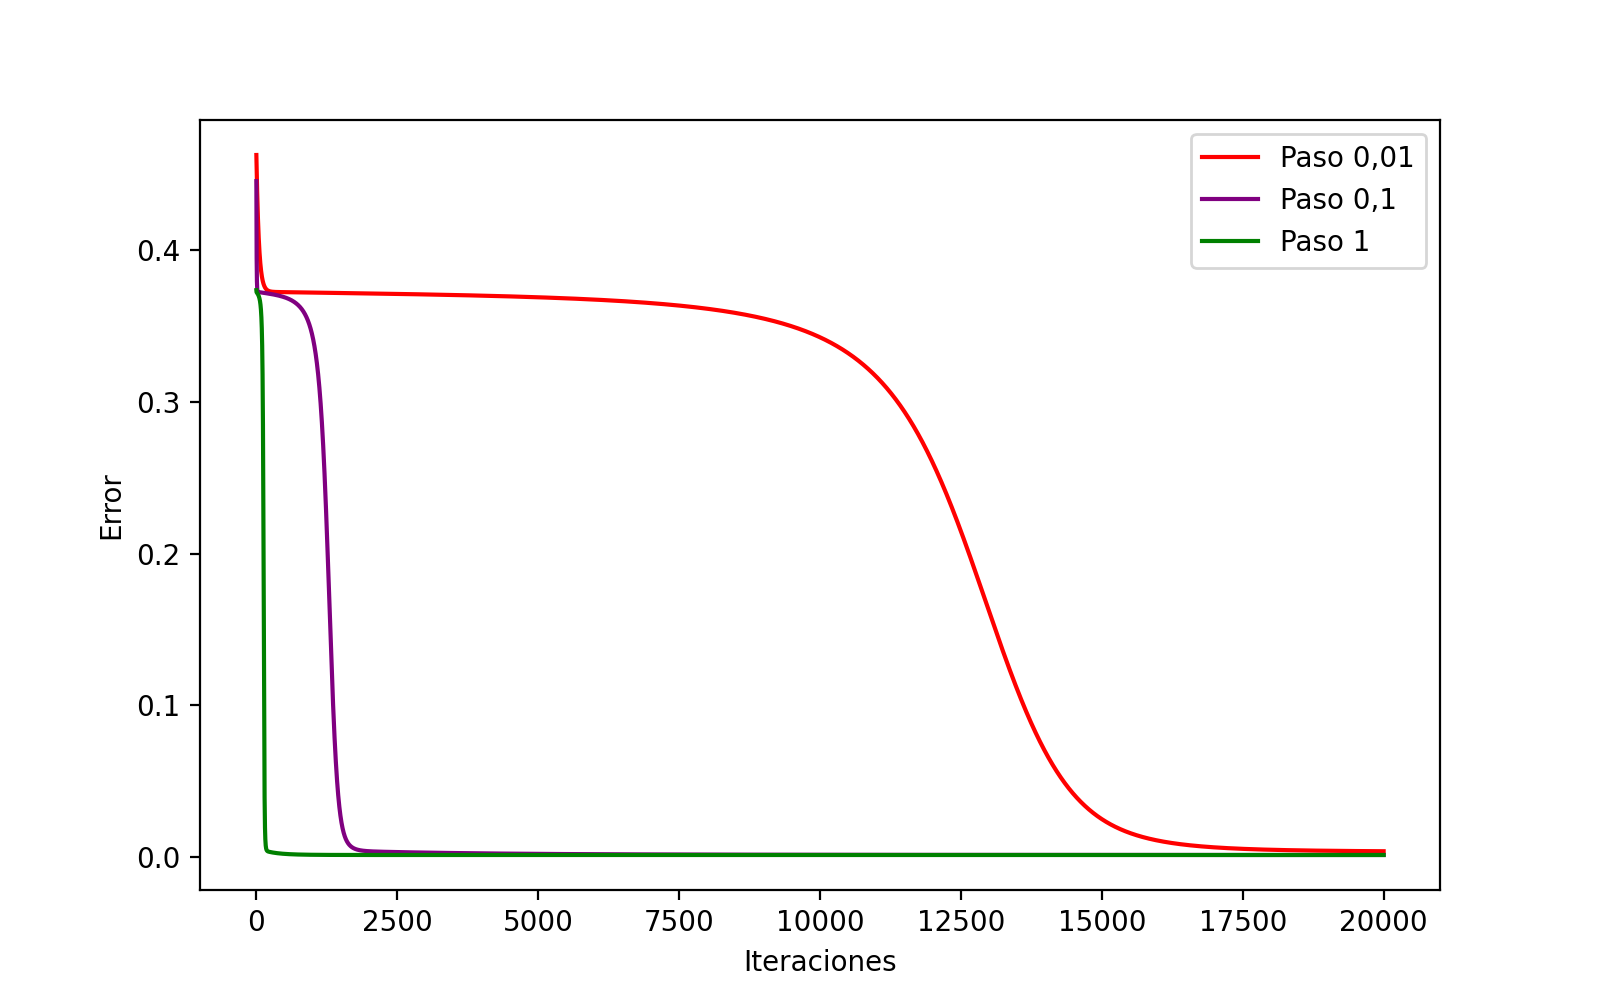
\includegraphics[width=0.5\textwidth]{figuras/figuras_p2/tres_curvas_error.png}
    \caption{Evolución errores de los 3 pasos más pequeños}
    \label{fig:cuatro_error}
\end{figure}

  Cuando el paso es muy grande, el error aumenta de forma veloz y nunca se acerca al valor esperado, mientras que el paso más pequeño reduce el error lentamente, los pasos más cercanos a 1 parecen ser los que reducen el error a una mayor velocidad

\newpage

\item \textbf{Distintas inicializaciones.}

  Repetimos d) con $\alpha = 1$, pero ahora utilizando 10 inicializaciones distintas entre [-1, 1] y otrad 10 entre [-5, 5]
  Los errores obtenidos fueron:
  \begin{tabular}{r l}
$\theta_0 \in [-1,1]$ & $\theta_0 \in [-5,5]$ \\
0.0013955411621448908 & 0.0014451338507139248 \\
0.001395355166404074 & 0.0013924007734941698 \\
0.0013954968993459397 & 0.0013988754077034768 \\
0.0014107347943005208 & 0.0014085433050804988 \\
0.0014059993258779813 & 0.0014211774414186044 \\
0.001416276508584076 & 0.001479627709811132 \\
0.0014153748402427463 & 0.37248297413788406 \\
0.001409257906983144 & 0.001400460223499488 \\
0.0014076924339753395 & 0.0014261599687102303 \\
0.0014149900866107252 & 0.0013918742850255864 \\
\end{tabular}


  (El orden no es importante ya que no hay relación entre las columnas)

  Como podemos ver, no siempre se alcanza el mismo valor de J, sin embargo, se alcanza valores similares, incluso iguales hasta la centésima, de modo que vemos que la aproximación es correcta
  Sin embargo [-5,5] presenta errores mayores, lo que se debe a que al tener un |t| grande la función σ′(t) se asemeja demasiado a cero lo que afecta a la resta en el cálculo de la gradiente, evitando que el valor varíe adecuadamente
  El descenso no garantiza alcanzar el mínimo global de J, ya que no es seguro que la aproximación llegue a ser exacta, sin importar cuanto se asemeje al valor esperado.

\end{enumerate}
\despueslista

\seccion{(g) Datos de otra función}

\begin{enumerate}[label=\roman*., widest=ii]
  \item \textbf{Entrenamiento.}

  \pendiente

  \item \textbf{Monotonía, cotas y por qué la red no puede aproximar $\tilde{f}$.}

  **1. Demostración de monotonía de $\hat{y}(x;\theta)$**

Sabemos por la definición de la red que la función de predicción es:
$$ \hat{y}(x; \theta) = c + v \cdot \sigma(a_2 \cdot \sigma(a_1x + b_1) + b_2) $$

Si derivamos $\hat{y}$ con respecto a $x$ aplicando la regla de la cadena (como se calculó en el inciso b), obtenemos:
$$ \frac{d\hat{y}}{dx} = v \cdot \sigma'(z_2) \cdot a_2 \cdot \sigma'(z_1) \cdot a_1 $$
*(Donde $z_1 = a_1x + b_1$ y $z_2 = a_2\sigma(z_1) + b_2$)*.

En el inciso (a) demostramos que la derivada de la función sigmoide es siempre estrictamente positiva ($0 < \sigma'(t) \le \frac{1}{4}$). Dado que $\sigma'(z_1) > 0$ y $\sigma'(z_2) > 0$ para cualquier valor de $x$, el signo de la derivada $\frac{d\hat{y}}{dx}$ depende exclusivamente del producto de los parámetros constantes: $(v \cdot a_2 \cdot a_1)$.

Dado que $v, a_2$ y $a_1$ son constantes fijas para un $\theta$ dado, su producto no puede cambiar de signo. En consecuencia, la derivada no cambia de signo en todo $\mathbb{R}$, lo que demuestra que la función $x \mapsto \hat{y}(x;\theta)$ es **estrictamente monótona** (siempre creciente o siempre decreciente dependiendo del signo del producto $v \cdot a_2 \cdot a_1$).

**2. Demostración de los límites de la salida**

La última capa de la red neuronal está definida como:
$$ \hat{y} = c + v \cdot h_2 $$
Donde $h_2 = \sigma(z_2)$. 

Sabemos que el recorrido de la función de activación sigmoide es estrictamente el intervalo abierto $(0, 1)$. Por lo tanto, $0 < h_2 < 1$. 
Si evaluamos los casos extremos para $h_2$:
* Cuando $h_2 \to 0$, $\hat{y} \to c + v(0) = c$.
* Cuando $h_2 \to 1$, $\hat{y} \to c + v(1) = c + v$.

De esto concluimos que, independientemente del valor de entrada $x$ o de los parámetros $\theta$, la predicción de la red $\hat{y}$ está siempre **acotada** en el intervalo comprendido entre $c$ y $c+v$.

**3. Conclusión sobre el ajuste a los nuevos datos $\tilde{f}$**

Al observar el gráfico de dispersión del inciso (g.i), los nuevos datos $\tilde{f}$ tienen un comportamiento claramente **no monótono** en el intervalo $[-1, 1]$ (la curva sube hasta formar un pico y luego desciende). 

Como se demostró en los puntos anteriores, la arquitectura de esta red neuronal específica (dos capas ocultas con una sola neurona cada una) solo tiene la capacidad matemática de representar funciones que sean **estrictamente monótonas y acotadas**. 

Debido a esta limitación estructural, la red es incapaz de "doblarse" para reflejar subidas y bajadas. Por lo tanto, es matemáticamente imposible que esta red se ajuste de forma correcta a la función $\tilde{f}$, sin importar cuántas iteraciones se realicen en el entrenamiento, el tamaño del paso ($\alpha$) elegido o los valores de inicialización ($\theta_0$).
\end{enumerate}

\end{document}
